\chapter{Two levels system}
\label{ch:TLS}

\section{Two-levels systems admit negative temperatures}
The simplest system that can exhibit negative temperatures is the two levels system (TLS). \\
A TLS is a system, for example a particle, for which only two values of energy are admitted, say $E_1$ and $E_2$. Let us denote the 
corresponding eigenstates by $\ket{1}$ and $\ket{2}$. An example of such a system, which we may consider in the following derivations, can be a spin-$1/2$ fermion in a uniform magnetic field.
Let us now consider a system composed of $N$ TLS. It is convenient to introduce the occupation numbers $n_1, n_2$ which denote,
respectively, the number of TLS at energy $E_1$ and $E_2$. If we set $E_1=\epsilon$ and $E_2=0$ for simplicity, the energy of the system is
\begin{equation}
    E = n_1 E_1 + n_2 E_2 = n_1\epsilon
    \label{eq:TLS_ensemble_energy}
\end{equation}
where $n_1 + n_2 = N$. \\
One macrostate of the system is thus identified by its energy and the total number of particles. The number of microstates corresponding 
to one given macrostate is the number of ways in which one can rearrange the particles in a way such that the total energy remains fixed, that is 
\begin{equation*}
    \Omega(E, N) = \frac{N!}{n_1!n_2!} = \frac{N!}{n_1! \, (N-n_1)!}
\end{equation*}
which corresponds to the Boltzmann entropy 
\begin{equation}
    S(E, N) = k_B\ln\left(\frac{N!}{n_1! \, (N-n_1)!}\right)
    \label{eq:TLS_entropy_N}
\end{equation}
In the limit of large $N$ the last expression can be expanded by using the Stirling's formula $\ln(N!) \approx N\ln N - N$ which yields 
\begin{equation}
    S(E, N) \approx N \ln \left(\frac{N}{N-n_1}\right) + n_1 \ln\left(\frac{N-n_1}{n_1}\right)
    \label{eq:TLS_entropy_N_approx}
\end{equation}
By using relation \ref{eq:TLS_ensemble_energy}
\begin{equation}\begin{gathered}
    \frac{1}{T} = \frac{\partial S}{\partial E} = \frac{\partial S}{\partial n_1} \, \frac{\partial n_1}{\partial E} =
    \frac{k_B}{\epsilon} \, \ln\left(\frac{N - n_1}{n_1}\right) = -\frac{k_B}{\epsilon} \, \ln\left(\frac{E}{N\epsilon - E}\right)
\end{gathered} 
\label{eq:T_tls} 
\end{equation}
where in the last step I used equation \ref{eq:TLS_ensemble_energy} again inside the logarithm's argument. \\
A plot of the temperature as a function of the system's energy is reported in figure \ref{fig:temperature_TLS}. Negative temperatures occur in the region in which $E > \frac{N\epsilon}{2}$, which corresponds to the states in which there are more particles 
in the excited state than in the lower one. As mentioned at the end of chapter \ref{ch:temperature}, negative temperatures occur above $+\infty$ rather than below the absolute zero. When a TLS is cooled down to $\SI{0}{\degree\kelvin}$ all the spins lie in the ground state, i.e. the state of minimum energy.
As soon as one adds energy to the system, the temperature starts increasing and more and more particles get excited to the higher energy state untill the point in which, on average, we expect the particles to be half excited and half in the ground state, that is we have the same probability 
of having an excited particle or a particle in the ground state. This happens when the temperature is ideally infinite, either positive or negative, and this constitutes the state of maximum entropy. By keeping adding energy to the system one ends up having more particles in the excited state rather than in the lower one,
experiencing the \emph{population inversion}. \\
\begin{figure}[h]
    \centering 
    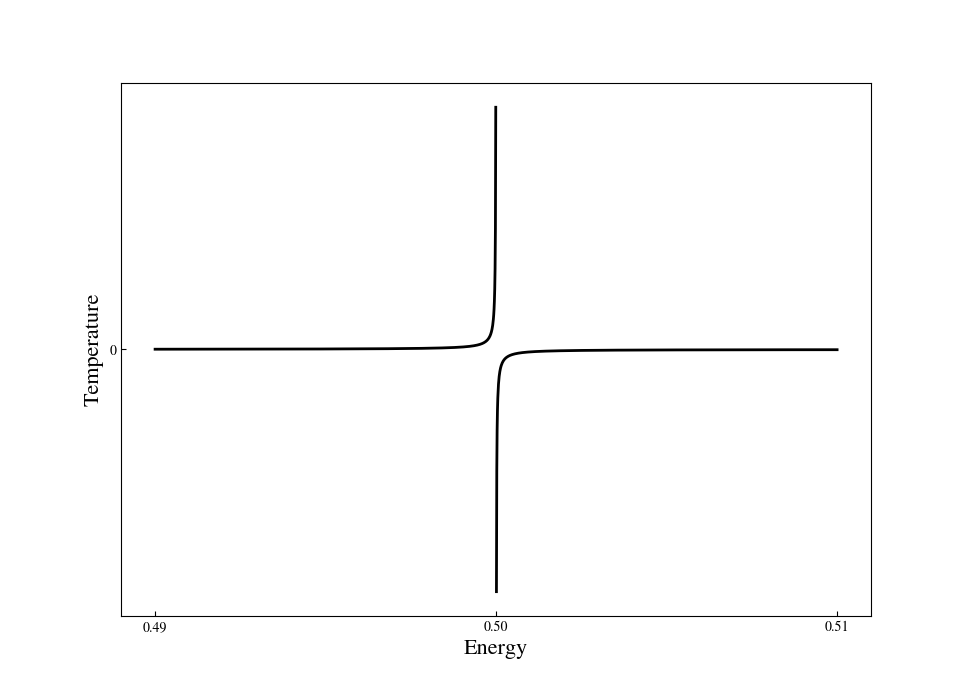
\includegraphics[scale=0.65]{images/temperature_TLS.png}
    \caption{The plot reports the temperature as a function of the energy ($E/N\epsilon$) in a two-levels system. When there are more excited particles than those in the lower state (energy $> 0.5$), the system exhibits negative absolute temperatures.}
    \label{fig:temperature_TLS}
\end{figure}
Equation \ref{eq:T_tls} can be rewritten as
\begin{equation*}
    \frac{1}{T} = \frac{k_B}{\epsilon} \ln\left(\frac{n_2}{n_1}\right)
\end{equation*}
which leads to 
\begin{equation}
    \frac{n_1}{n_2} = e^{-\epsilon/k_BT}
    \label{eq:spin_temperature}
\end{equation}
This formula allows us to introduce the so called \emph{spin temperature}. \\
In the derivation of the results for the two level system we implicitly assume that the spin system is
isolated from the environment and that the spins do not interact each other or, in other words, that each spin is isolated from the rest of the thermodynamic universe.
In practice this is not the case and in general such a system is described by a Hamiltonian of the type
\begin{equation}
    \mathcal{H} = \mathcal{H}_0 + \mathcal{H}_{ss} + \mathcal{H}_{sl}
    \label{eq:Hamiltonian_lattice_spin}
\end{equation}
where $H_0$ represents the single particle Hamiltonian implicitly assumed in the previous derivation, $H_{ss}$ represents the spin-spin interaction and $H_{sl}$ represents the spin-lattice interaction. \\
The term $H_{ss}$ can be conveniently considered negligible but cannot be zero: indeed this therm plays a fundamental role for guaranteeing the \emph{ergodicty} of the system. \\
The spin-lattice interaction on the other side can be characterized by a typical interaction time $\tau_L$. The time $\tau_L$ characterizes the speed under which the spins adapts to a change in the lattice temperature. 
When the observation time of the experiment $\tau_s$ is much smaller than the typical interaction time $\tau_s \ll \tau_L$ the change in the system due to the spin-lattice interaction is negligible and equation \ref{eq:spin_temperature} defines a temperature which is dependent only on the spins' configuration. \\
We call this temperature \emph{spin temperature} \cite{Spin_temperature}: Note that for $t\ll \tau_L$ this temperature may differ by the one of the lattice while for $t \gg \tau_L$ the two temperatures coincide. \par
\vspace{10pt}
Let us now recall what we mentioned at the end of chapter \ref{ch:temperature}: a system whose maximum energy state is allowed by only one or few microstates may exhibit a decreasing entropy as a function of the energy, hence admitting negative temperatures. This is 
exactly the case of a TLS for which the maximum energy state corresponds to exactly one precise microstate, that is when all the particles are in the excited state. This of course corresponds to a null entropy. Analogously, the same happens at the minimum energy for which there is only 
one corresponding microstate and the entropy is null. For all the other states the entropy is non-zero and is given by formula \ref{eq:TLS_entropy_N_approx}. The whole expressions as a function of the energy can be easilly obtained by \ref{eq:TLS_entropy_N} by multiplying and diving by $\epsilon$ both inside and outside the logarithm
\begin{equation}
    S(E, N) / k_B = N \ln\left(\frac{N\epsilon}{N\epsilon - E}\right) + \frac{E}{\epsilon} \ln\left(\frac{N\epsilon - E}{\epsilon}\right)
    \label{eq:entropy_E_TLS}
\end{equation}
and is reported in figure \ref{fig:TLS_entropy_E}. \\
\begin{figure}[h]
    \centering 
    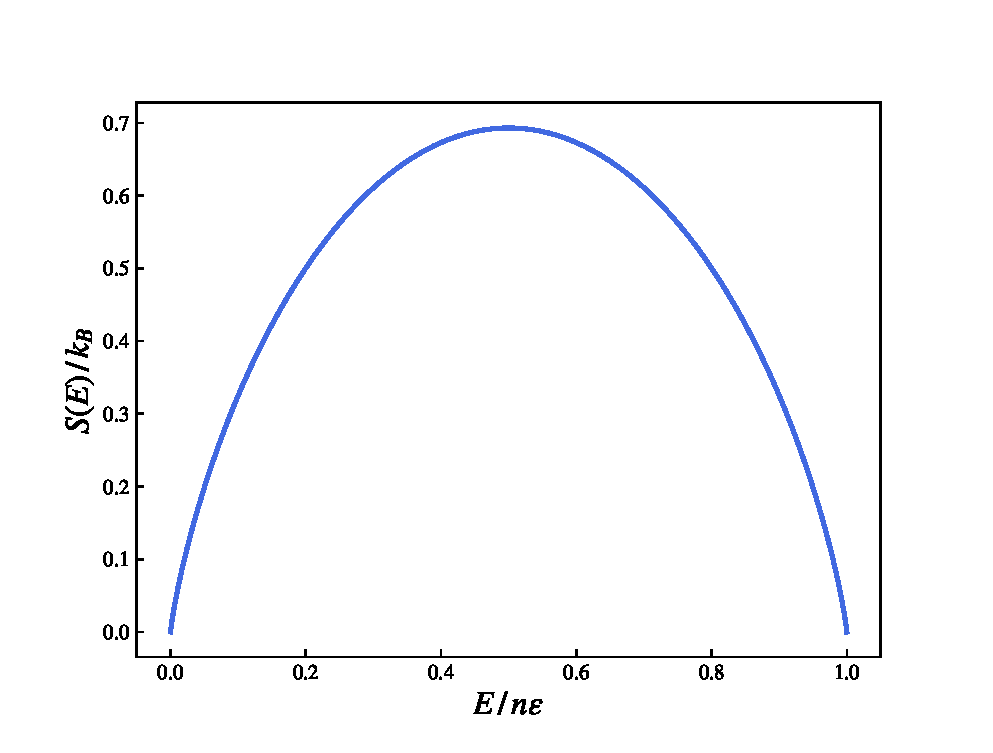
\includegraphics[scale=0.65]{images/entropy_TLS.eps}
    \caption{Entropy of a TLS as a function of the energy.}
    \label{fig:TLS_entropy_E}
\end{figure}
This insight can be formalized into \emph{Ramsey's criteria}.
\newpage
\section{Ramsey's criteria}
Ramsey \cite{Ramsey} provided 3 conditions under which a thermodynamic system exhibits negative temperatures
\begin{enumerate}
    \item \emph{The various elements of the thermodynamic system under analysis must be at equilibrium with each other}. \\
    This condition must be verified in order to define a temperature for the whole system.
    \item \emph{There must be an upper bound on the energy of the system} \\
    In fact it is known from statistical mechanics that the probability (or probability density) for the system to be in a state of energy $E$ is 
    \begin{equation}
        p(E) \propto e^{-\beta E}
        \label{eq:probability_ramsey}
    \end{equation}
    where $\beta = 1/k_BT$. If negative temperatures are admitted by the system and the latter does not admit an upper bound on the energy, the exponential factor in equation \ref{eq:probability_ramsey}
    becomes infinitely large for increasing energy. This means that if the system admits negative temperature, the higher the energy, the higher the probability of the system to be in that state. The most probable state 
    would then be the one at infinite energy making the other states negligible in probability. Clearly, an infinite amount of energy cannot be put into the system, meaning that such a system cannot exist.
    \item \emph{The thermodynamic system under analysis must be thermally isolated from other systems that do not satisfy the above conditions}. \\
    In good approximation one can think that the time required to reach equilibrium among the elements of the system is small compared to the time of interaction
    between the system and the environment or another system.
\end{enumerate}
The above conditions are all satisfied by the TLS described above. Indeed it admits negative temperatures. \\